\documentclass[11pt,a4paper]{article}
\usepackage{jheppub}
\usepackage{amsmath,amssymb,booktabs,array,multirow}
\usepackage{xcolor}
\usepackage{microtype}
\usepackage{graphicx}

\newcommand{\Herwig}{\textsc{Herwig}}
\newcommand{\Rivet}{\textsc{Rivet}}
\newcommand{\ap}{A_{\parallel}}
\newcommand{\al}{A_{L}}
\newcommand{\all}{A_{LL}}
\newcommand{\suu}{\sigma_{UU}}
\newcommand{\sll}{\sigma_{LL}}
\newcommand{\GeV}{\ensuremath{\,\mathrm{GeV}}}
\newcommand{\placeholderfigure}[2]{%
  \begin{figure}[t]
    \centering
    \fbox{\begin{minipage}[c][4.2cm][c]{0.88\textwidth}
      \centering\small\color{gray!70!black}
      Production-statistics placeholder\\[0.5em]
      #1
    \end{minipage}}
    \caption{#2 The numerical curves and uncertainty bands will be inserted
    after the production campaign; no quantitative conclusion is inferred
    from this placeholder.}
  \end{figure}}

\title{Phenomenological Investigations of Polarized Collisions in \Herwig~7}

\author[a]{Andreas Papaefstathiou}
\affiliation[a]{Department of Physics, Kennesaw State University,
830 Polytechnic Lane, Marietta, GA 30060, USA}
\emailAdd{apapaefs@kennesaw.edu}

\abstract{
We formulate a set of particle-level comparisons between the polarized-event
simulation in \Herwig~7 and measurements from fixed-target deep-inelastic
scattering and longitudinally polarized proton--proton collisions.  The
deep-inelastic-scattering study comprises inclusive proton and deuteron data
from HERMES and COMPASS together with identified-hadron semi-inclusive HERMES
measurements.  The proton--proton study considers weak-boson, inclusive-jet
and dijet production measured by STAR at centre-of-mass energies of 200 and
$510\GeV$.  Neutral-current deep-inelastic scattering is described at
next-to-leading order matched to the parton shower using the POWHEG method,
whereas the proton--proton hard processes are treated at leading order and
evolved with a spin-correlated parton shower.  We define the helicity
combinations, fiducial measurements and uncertainty prescriptions needed for
a reproducible comparison.  A first central-PDF scale scan is presented for
inclusive DIS and weak-boson production; the jet and semi-inclusive results
remain provisional pending production statistics.
}

\begin{document}
\maketitle
\flushbottom

\section{Introduction}
\label{sec:introduction}

The spin structure of the proton is constrained by measurements that probe
different combinations of partonic helicities and different regions of
momentum fraction and scale.  Inclusive polarized deep-inelastic scattering
(DIS) remains the most direct source of information on quark helicity
distributions.  Longitudinally polarized proton--proton collisions at RHIC
provide complementary flavour sensitivity through parity-violating weak-boson
production and sensitivity to the gluon helicity distribution through
inclusive-jet and dijet production.  Semi-inclusive DIS adds flavour
information through identified hadrons and probes how the helicity-dependent
hard process is embedded in an exclusive hadronic final state.  A common
exclusive-event
description of these measurements is useful both as a test of the polarized
hard-scattering implementation and as a starting point for phenomenology in
which showering, hadronization, decays and the underlying event cannot be
cleanly separated from the observable definition.

The implementation of polarized DIS in \Herwig~7 was developed and validated
in ref.~\cite{Masouminia:2026pol}.  That work introduced an NLO treatment based
on POWHEG matching and a spin-correlation prescription that initializes the
parton shower from the Born spin-density matrix and, when requested, propagates
the spin information associated with an accepted real-emission
configuration.  Integrated rates were compared with fixed-order calculations,
and shower-sensitive observables were used to isolate the effects of the
different spin treatments.  The present study changes the emphasis from
internal validation to comparison with published measurements.  It also
extends the scope to polarized proton--proton reactions.

The selected DIS data are the HERMES inclusive proton measurement at a
positron energy of $27.6\GeV$~\cite{HERMES:2006}, the HERMES identified-hadron
semi-inclusive measurements on proton and deuteron targets at the same beam
energy~\cite{HERMES:2019sidis}, the COMPASS proton measurements at nominal
muon energies of 160 and $200\GeV$~\cite{COMPASS:2010,COMPASS:2015}, and the
COMPASS deuteron measurement at $160\GeV$~\cite{COMPASS:2016d}.  The RHIC
measurements are the STAR single- and double-spin asymmetries in
$W^\pm$ production and the integrated single-spin asymmetry in
$Z/\gamma^*$ production~\cite{STAR:2018}, together with inclusive-jet and
dijet double-spin asymmetries at 200 and
$510\GeV$~\cite{STAR:2021jets,STAR:2022jets}.  Particle- and parton-level
measurements are constructed with the conventions of
\Rivet~\cite{Bierlich:2019rhm}.

Throughout this work the unpolarized proton densities are taken from the NLO
NNPDF4.0 set~\cite{NNPDF:2021} and helicity differences from NNPDFpol2.0 at
NLO~\cite{NNPDFpol:2025}.  This pairing is used even for the leading-order RHIC
matrix elements in order to maintain a common partonic input across the
study; it does not promote those predictions to NLO accuracy.  An important
qualification is that NNPDFpol2.0 includes much of the HERMES, COMPASS and
STAR information considered here.  Agreement with those measurements is
therefore not an independent validation of the polarized PDF fit.  It tests
instead the consistency of the hard process, helicity bookkeeping and
exclusive event evolution with the fitted information.

The paper is organized as follows.  Section~\ref{sec:dis} defines the
inclusive and semi-inclusive DIS observables, simulation and experimental
selections.  Section~\ref{sec:pp} describes weak-boson and jet production in
polarized proton--proton collisions.  Provisional conclusions are given in
section~\ref{sec:conclusions}.  The low-$Q^2$ HERMES projection and compact
reproducibility tables are collected in the appendices.

\section{Deep-inelastic scattering}
\label{sec:dis}

\subsection{Helicity cross sections and observables}

We use four independent samples with unit longitudinal beam and target
helicities, denoted by $PP,PM,MP,MM$.  Their normalized differential cross
sections are combined as
\begin{align}
  \suu &= \frac{1}{4}\left(\sigma_{PP}+\sigma_{PM}
              +\sigma_{MP}+\sigma_{MM}\right),
  \\
  \sll &= \frac{1}{4}\left(\sigma_{PP}-\sigma_{PM}
              -\sigma_{MP}+\sigma_{MM}\right).
  \label{eq:dis-combinations}
\end{align}
The longitudinal lepton--nucleon asymmetry is
$\ap=\sll/\suu$.  The virtual-photon asymmetry is related to the measured
quantity by
\begin{equation}
  \ap = D\left(A_1+\eta A_2\right),
  \label{eq:depolarization}
\end{equation}
where $D$ is the longitudinal depolarization factor.  We set
$A_2=g_2=0$, so the prediction for $A_1$ is obtained by weighting the
polarized cross section with $1/D$ before forming the ratio.  This operation
is performed event by event; replacing $D$ by a bin-centre value would not
give an equivalent prediction.  R1990 is used in the HERMES depolarization
factor and R1998 in the COMPASS factor.  The finite incoming-muon mass is kept
for COMPASS.

The four unit-helicity samples, rather than finite experimental beam and
target polarizations, define the theory prediction.  This removes dependence
on the polarization and dilution corrections used by an experiment to unfold
its published asymmetry.  It also provides the parity diagnostics
$PP-MM$, $PM-MP$, and the corresponding single-spin combinations.  Empty
denominators are left undefined.  For NLO samples, positive- and
negative-weight perturbative components are summed after each has been
normalized and after all shards have been combined, but before
eq.~\eqref{eq:dis-combinations} is evaluated.

\subsection{Event simulation}

Neutral-current DIS is generated through pure photon exchange with the
polarized NLO matrix elements of \Herwig~7.3~\cite{Bewick:2023tfi}.  The hard
process is matched to the angular-ordered parton shower using the POWHEG
method~\cite{Nason:2004rx,Frixione:2007vw}.  The nominal prediction includes
the QCD shower, spin correlations, cluster hadronization, unstable-particle
decays and beam-remnant treatment.  QED shower radiation and multiple-parton
interactions are switched off for these fixed-target measurements.  The
generation window is aligned with the DIS selection to avoid relying on a
post-generation rejection of most events.

The central Born factorization and renormalization scales are set by the
photon virtuality, while the POWHEG emission uses the corresponding native
hardest-emission scales.  A common variation factor
$\mu/\mu_0=1/2,1,2$ is applied consistently to the supported
factorization, renormalization and emission scales.  No scale is evaluated
below $1\GeV$.  This lower boundary coincides with the scale limit of the
chosen PDF grids and is especially relevant for the HERMES projection in
appendix~\ref{app:lowq2}.

Five simulation variants are retained for the DIS comparison:
\begin{enumerate}
  \item the nominal polarized NLO+PS prediction with the complete spin
  treatment;
  \item NLO+PS with unpolarized incoming beams, used as a closure test;
  \item polarized LO+PS;
  \item polarized NLO+PS in which the accepted real emission does not supply
  an additional spin-density matrix; and
  \item polarized NLO+PS with shower spin correlations disabled.
\end{enumerate}
The last three are diagnostics, not components of the nominal uncertainty
band.  In particular, the comparison without real-emission spin information
does not alter the POWHEG hardest-emission probability or event weight.

\subsection{HERMES proton data}

The primary HERMES observable is the published 15-bin $A_1^p(x)$
measurement with $1<Q^2<20\,\mathrm{GeV}^2$.  Laboratory kinematics are
reconstructed from the incoming and outgoing positron momenta and the target
four-momentum,
\begin{equation}
 Q^2=-q^2,\qquad
 x=\frac{Q^2}{2P\mathbin{\cdot}q},\qquad
 y=\frac{P\mathbin{\cdot}q}{P\mathbin{\cdot}k},\qquad
 W^2=(P+q)^2 .
\end{equation}
The selection requires $0.1<y\leq0.91$,
$W^2>3.24\,\mathrm{GeV}^2$, and a positron scattering angle
$0.04\leq\theta\leq0.22$.  The lower edge $Q^2=1\,\mathrm{GeV}^2$
is exactly the PDF-grid boundary and is consequently treated as an
exploratory region.  A nested $Q^2>4\,\mathrm{GeV}^2$ selection provides a
more conservative validation view.

The same publication also provides a 45-point Born-level
$\ap(x,Q^2)$ projection in 19 $x$ slices.  It is scientifically distinct
from the primary $A_1^p(x)$ comparison and is discussed separately in
appendix~\ref{app:lowq2}.

\subsection{HERMES identified-hadron semi-inclusive data}
\label{sec:hermes-sidis}

The semi-inclusive HERMES measurement reports longitudinal double-spin
asymmetries for identified charged pions and kaons produced on proton and
deuteron targets~\cite{HERMES:2019sidis}.  We use a $27.6\GeV$ positron beam
and pure photon exchange.  Within this one-photon approximation the same
prediction represents the combined electron and positron sample.  In addition
to the inclusive variables, the hadron kinematics are characterized by
\begin{equation}
 z=\frac{P\mathbin{\cdot}p_h}{P\mathbin{\cdot}q},
 \qquad P_{hT}=|\boldsymbol p_h-(\boldsymbol p_h\mathbin{\cdot}
 \hat{\boldsymbol q})\hat{\boldsymbol q}|,
\end{equation}
together with the Feynman variable $x_F$ in the photon--nucleon
centre-of-mass frame.

The DIS selection requires $Q^2>1\,\mathrm{GeV}^2$,
$W^2>10\,\mathrm{GeV}^2$, $y<0.85$, and
$0.04<\theta<0.22$.  Accepted hadrons satisfy $x_F>0.1$ and normally
$0.2<z<0.8$; the interval $0.1<z<0.2$ is retained only for the published
$x$--$z$ projection in which it appears.  The proton measurement uses
$\pi^\pm$ with $4<p_h<13.8\GeV$, whereas the deuteron measurement uses
$\pi^\pm$ and $K^\pm$ with $2<p_h<15\GeV$.  Every accepted identified hadron
contributes.  We retain the published nine-bin $x$ projection, the coarse
$x$--$z$ and $x$--$P_{hT}$ projections, and the three-dimensional
$x$--$z$--$P_{hT}$ grid.

Proton and neutron target components are generated separately.  The proton
sample is used both for the hydrogen result and for the proton component of
deuterium, with the corresponding hadron acceptance applied in each case.
The deuteron impulse approximation is
\begin{equation}
 \suu^d=\frac{\suu^p+\suu^n}{2},\qquad
 \sll^d=0.926\,\frac{\sll^p+\sll^n}{2}.
 \label{eq:sidis-deuteron}
\end{equation}
Charge-difference asymmetries are constructed from normalized yields,
\begin{equation}
 A_\parallel^{h^+-h^-}=
 \frac{\sll^{h^+}-\sll^{h^-}}
      {\suu^{h^+}-\suu^{h^-}},
 \label{eq:sidis-charge-difference}
\end{equation}
rather than by subtracting the two charge-separated asymmetries.  The primary
comparison is made directly to the published $A_\parallel$ values, so no
$A_2$, $g_2$, or depolarization model enters.  Since the one-, two- and
three-dimensional projections contain overlapping events and no
cross-projection covariance is published, they are assessed separately.

\placeholderfigure{HERMES proton $\pi^\pm$ and deuteron
$\pi^\pm,K^\pm$ $A_\parallel$ in the one-, two- and three-dimensional
published projections.}
{The HERMES identified-hadron SIDIS comparison.  The analysis and reference
data have passed the central validation run; production-statistics curves are
not inferred from the 100-event smoke sample.}

\subsection{COMPASS proton and deuteron data}

The 2010 proton measurement uses a nominal $160\GeV$ positive-muon beam and
15 bins in $0.004<x<0.7$.  We require $Q^2>1\,\mathrm{GeV}^2$ and
$0.1<y<0.9$, without imposing an additional hadronic-mass cut that is not
reported for this table.  Fixed-energy generation at $160\GeV$ approximates
the published 140--180 GeV beam-energy selection.  The later proton sample
uses a $200\GeV$ beam and extends the reach towards smaller $x$.

For the deuteron comparison, proton and neutron hard scatterings are generated
separately and combined in the impulse approximation.  The longitudinal
combination includes the effective nucleon polarization associated with the
deuteron $D$-state correction.  Nuclear modifications beyond this
approximation are not modeled.  As for the proton data, the published
$A_1^d$ is compared with the prediction obtained using $A_2=g_2=0$.

Table~\ref{tab:dis-selections} summarizes the principal selections.  Exact
published bin boundaries are used for every comparison.

\begin{table}[t]
  \centering
  \caption{Fixed-target DIS configurations.  The HERMES low-$Q^2$
  projection is detailed in appendix~\ref{app:lowq2}.}
  \label{tab:dis-selections}
  \small
  \begin{tabular}{@{}llllll@{}}
    \toprule
    Measurement & beam & target & observable & $Q^2\,[\mathrm{GeV}^2]$ & $y$ \\
    \midrule
    HERMES primary & $e^+,27.6\GeV$ & $p$ & $A_1^p(x)$ & $1--20$ & $0.1--0.91$ \\
    HERMES SIDIS & $e^+,27.6\GeV$ & $p,d$ & $A_\parallel^{\pi,K}$ & $>1$ & $<0.85$ \\
    COMPASS 2010 & $\mu^+,160\GeV$ & $p$ & $A_1^p(x)$ & $>1$ & $0.1--0.9$ \\
    COMPASS 2016 & $\mu^+,200\GeV$ & $p$ & $A_1^p(x)$ & $>1$ & published \\
    COMPASS 2017 & $\mu^+,160\GeV$ & $d$ & $A_1^d(x)$ & $1--100$ & published \\
    \bottomrule
  \end{tabular}
\end{table}

\subsection{Uncertainties and presentation}

The nominal curve carries separate Monte Carlo, PDF and hard-scale
uncertainties.  Polarized PDF replicas are varied while the unpolarized member
is held central, and conversely for unpolarized replicas.  A single replica
member is used coherently in every helicity and in both signed NLO
components.  The two independent replica variances are then added in
quadrature to form the 68\% PDF band.  The scale envelope is not combined with
the PDF or Monte Carlo uncertainty.

The plots display one total experimental uncertainty per point.  Monte Carlo
statistical uncertainties form a theory-centred band, separate from the
hard-scale envelope.  For asymmetries near zero, pulls using the combined
experimental and Monte Carlo statistical uncertainty are more stable than
data/theory ratios.  The overlap between the experimental inputs and the
NNPDFpol2.0 fit is stated on all quantitative summaries.

Figure~\ref{fig:inclusive-dis-data} shows the completed central-PDF scale
scan.  Each DIS scale point contains 300,000 positive NLO events and 30,000
negative NLO events for every physical helicity and, for deuterium, every
nucleon component.  The PDF-replica ensemble is not part of this first scan
and is therefore not drawn.  The common rise of the proton asymmetry with
$x$ is reproduced across the three beam configurations.  The deuteron
prediction remains close to zero at small $x$ and becomes positive at larger
$x$, following the broad trend of the data.  The lowest-$x$ bins also show
that scale and Monte Carlo uncertainties can be appreciable when the
polarized numerator is small; these bins should not be read as a precision
test of the shower.

\begin{figure}[p]
  \centering
  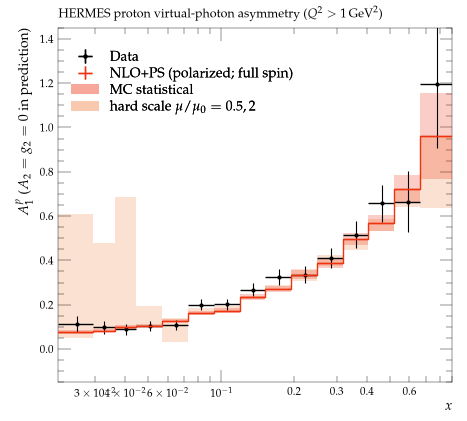
\includegraphics[width=0.48\textwidth]{figures/scan-20260722/dis/hermes-a1.png}
  \hfill
  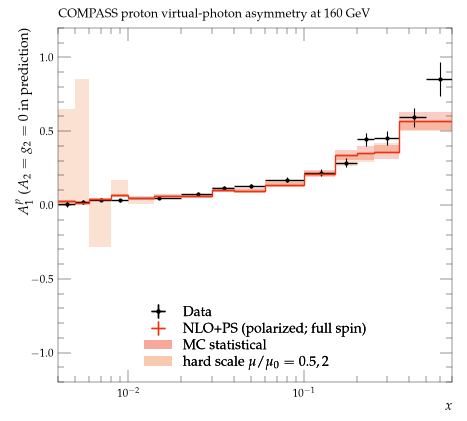
\includegraphics[width=0.48\textwidth]{figures/scan-20260722/dis/compass-2010-a1.png}

  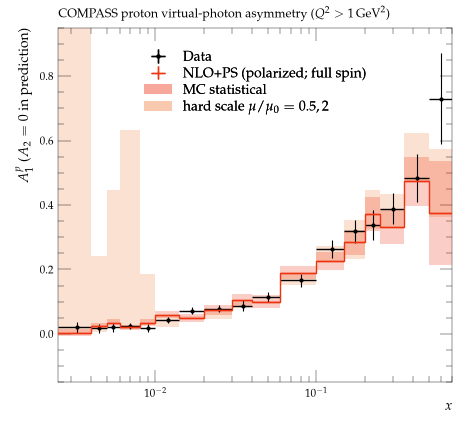
\includegraphics[width=0.48\textwidth]{figures/scan-20260722/dis/compass-2016-a1.png}
  \hfill
  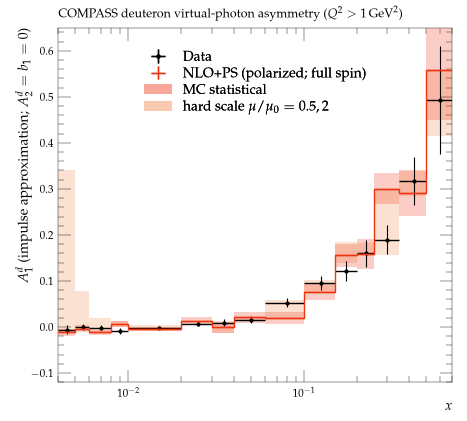
\includegraphics[width=0.48\textwidth]{figures/scan-20260722/dis/compass-2017-a1.png}
  \caption{Inclusive virtual-photon asymmetries from the central-PDF
  production scan.  Top left: HERMES proton data at $27.6\GeV$.  Top right:
  COMPASS proton data at $160\GeV$.  Bottom left: COMPASS proton data at
  $200\GeV$.  Bottom right: COMPASS deuteron data at $160\GeV$.  The red
  stepped curve is the nominal polarized NLO+PS prediction.  The
  theory-centred red band is its Monte Carlo statistical uncertainty and the
  lighter envelope is the common hard-scale variation
  $\mu/\mu_0=1/2,1,2$.  The experimental points carry their published total
  uncertainties.  The $A_1$ construction uses $A_2=g_2=0$.}
  \label{fig:inclusive-dis-data}
\end{figure}

\section{Proton--proton collisions}
\label{sec:pp}

\subsection{Common simulation and spin combinations}

The STAR measurements are simulated in longitudinally polarized
proton--proton collisions at $\sqrt{s}=200$ or $510\GeV$.  Four independently
generated helicity samples are again used.  With the first and second beam
helicities denoted by $h_1,h_2=\pm1$, the double-spin numerator follows the
same sign pattern as eq.~\eqref{eq:dis-combinations}.  The two single-beam
estimators are
\begin{align}
 A_L^A &=
 \frac{\sigma_{PP}+\sigma_{PM}-\sigma_{MP}-\sigma_{MM}}
      {\sigma_{PP}+\sigma_{PM}+\sigma_{MP}+\sigma_{MM}},\\
 A_L^B &=
 \frac{\sigma_{PP}-\sigma_{PM}+\sigma_{MP}-\sigma_{MM}}
      {\sigma_{PP}+\sigma_{PM}+\sigma_{MP}+\sigma_{MM}}.
 \label{eq:single-beam}
\end{align}

The weak-boson and QCD $2\to2$ hard matrix elements are leading order.  The
incoming partons are sampled with NNPDF40 NLO and NNPDFpol2.0 NLO, but all
RHIC predictions are labelled LO+PS.  Weak-boson production uses the combined
QCD and QED shower, spin-correlated decays, hadronization, beam remnants, and
multiple-parton interactions.  The primary jet prediction instead uses the
QCD shower and clusters hard shower partons before hadronization, with
multiple-parton interactions and QED showering disabled.  Stable-particle
jets with multiple-parton interactions form a separate modelling diagnostic.

The common hard-scale points are
$\mu/\mu_0=1/2,1,2$.  For electroweak Born $W/Z$ production only the
factorization scale is varied.  Jet production varies the supported
renormalization and factorization scale together.  PDF replicas are combined
with the same coherence and quadrature prescription as in DIS.

\subsection{STAR weak-boson asymmetries}

The $W^+$ and $W^-$ observables use prompt dressed positrons and electrons,
respectively.  Photons are recombined within $R=0.1$, and the dressed lepton
is required to satisfy
\begin{equation}
  25<E_T<50\GeV,\qquad -1.5<\eta_e<1.5.
\end{equation}
The result is evaluated in six bins of width 0.5.  Since the two RHIC beams are
physically equivalent, the measured single-spin asymmetry is formed from both
beam estimators,
\begin{equation}
 A_L(\eta)=\frac{1}{2}\left[A_L^A(\eta)+A_L^B(-\eta)\right].
 \label{eq:star-symmetrization}
\end{equation}
The published point coordinates are retained rather than replaced by bin
centres.  The $W^\pm$ double-spin asymmetry is obtained from all four
helicity samples, with mirrored pseudorapidity bins folded at normalized-yield
level.

For $Z/\gamma^*$ production we require two isolated, oppositely charged
dressed electrons with
\begin{equation}
 E_T>14\GeV,\qquad |\eta_e|<1.1,\qquad
 70<m_{ee}<110\GeV .
\end{equation}
The comparison is made with the integrated value
$A_L=-0.04\pm0.07$.  Because weak interactions violate parity, the relevant
closure test is the beam-exchange relation
\begin{equation}
 \sigma_{h_1h_2}(\eta)=\sigma_{h_2h_1}(-\eta),
 \label{eq:beam-exchange}
\end{equation}
rather than equality of $PP$ and $MM$.

The central-PDF scale scan contains 300,000 events per channel, helicity and
scale point.  Figure~\ref{fig:star-weak-data} shows all five published
weak-boson observables.  The LO+PS prediction reproduces the opposite signs
and broad pseudorapidity dependence of the $W^+$ and $W^-$ single-spin
asymmetries.  Most points are described within their total uncertainties,
although the pull panels in fig.~\ref{fig:star-weak-pulls} identify localized
deviations in both charge channels.  The predicted double-spin asymmetries are
positive across the fiducial region, while the measured central values lie
closer to zero and have substantially larger uncertainties.  The integrated
$Z/\gamma^*$ prediction is close to the measured central value.  These
comparisons test the exclusive LO+PS realization of the fitted helicity
information; they do not constitute an independent validation of the
NNPDFpol2.0 fit.

\begin{figure}[p]
  \centering
  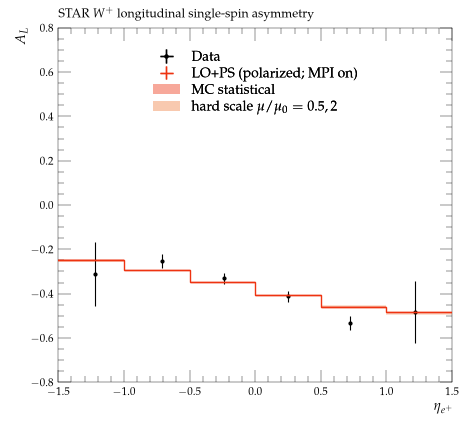
\includegraphics[width=0.48\textwidth]{figures/scan-20260722/star-weak/wplus-al.png}
  \hfill
  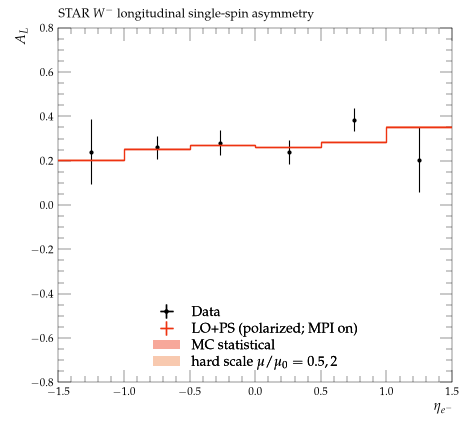
\includegraphics[width=0.48\textwidth]{figures/scan-20260722/star-weak/wminus-al.png}

  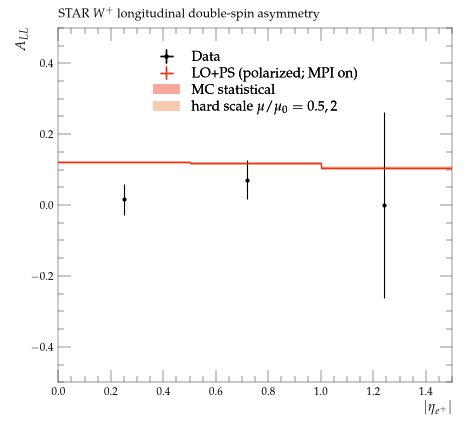
\includegraphics[width=0.48\textwidth]{figures/scan-20260722/star-weak/wplus-all.png}
  \hfill
  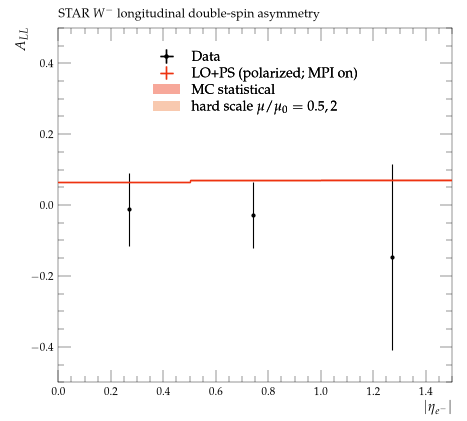
\includegraphics[width=0.48\textwidth]{figures/scan-20260722/star-weak/wminus-all.png}
  \caption{STAR $W^\pm$ spin asymmetries at $\sqrt{s}=510\GeV$.  The upper
  row shows $A_L$ for $W^+$ (left) and $W^-$ (right); the lower row shows the
  corresponding $A_{LL}$.  The red stepped curve is the polarized LO+PS
  prediction with multiple-parton interactions enabled.  The dark
  theory-centred band is the Monte Carlo statistical uncertainty and the
  lighter band is the factorization-scale envelope.  Experimental points
  carry their published total uncertainties.}
  \label{fig:star-weak-data}
\end{figure}

\begin{figure}[p]
  \centering
  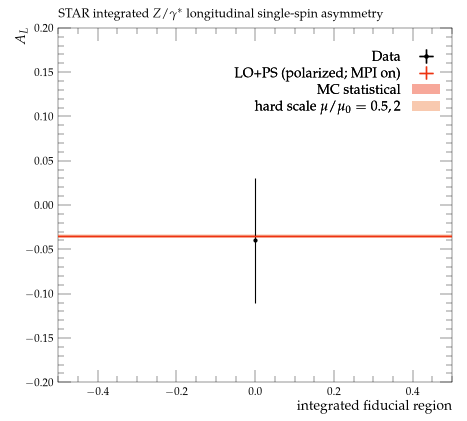
\includegraphics[width=0.58\textwidth]{figures/scan-20260722/star-weak/zgamma-al.png}
  \caption{The integrated STAR $Z/\gamma^*$ longitudinal single-spin
  asymmetry.  The line and uncertainty conventions are those of
  fig.~\ref{fig:star-weak-data}.}
  \label{fig:star-z-data}
\end{figure}

\begin{figure}[p]
  \centering
  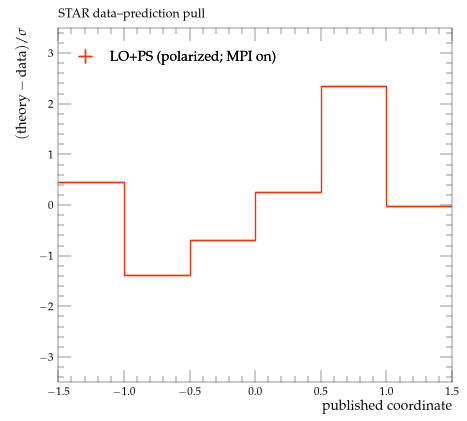
\includegraphics[width=0.46\textwidth]{figures/scan-20260722/star-weak/pull-wplus-al.png}
  \hfill
  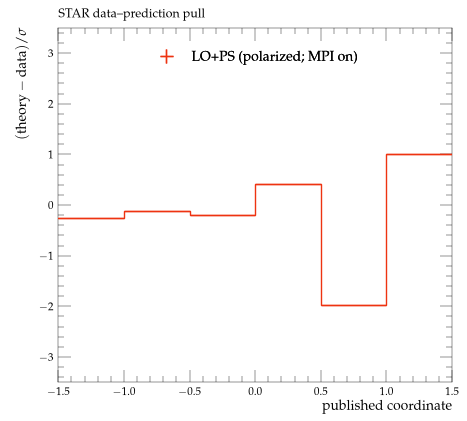
\includegraphics[width=0.46\textwidth]{figures/scan-20260722/star-weak/pull-wminus-al.png}

  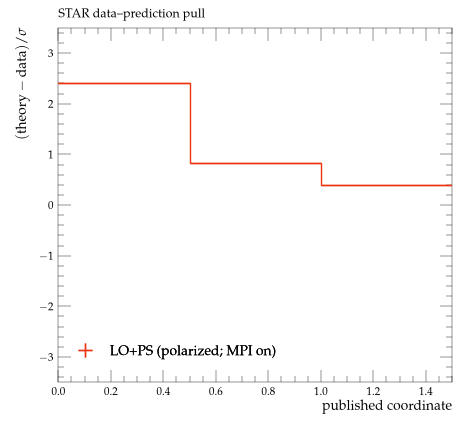
\includegraphics[width=0.46\textwidth]{figures/scan-20260722/star-weak/pull-wplus-all.png}
  \hfill
  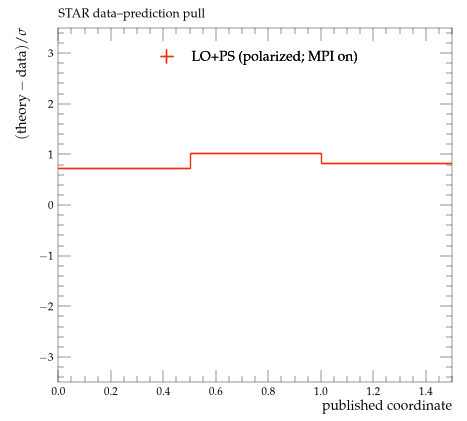
\includegraphics[width=0.46\textwidth]{figures/scan-20260722/star-weak/pull-wminus-all.png}

  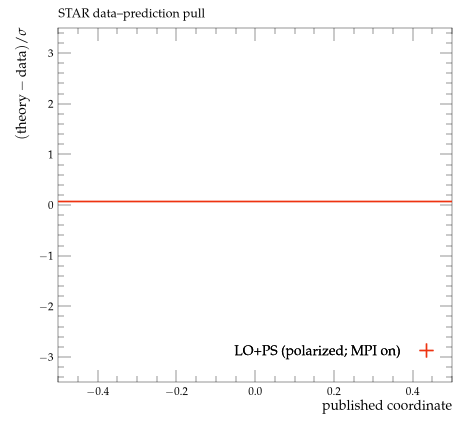
\includegraphics[width=0.48\textwidth]{figures/scan-20260722/star-weak/pull-zgamma-al.png}
  \caption{Pulls corresponding to the STAR weak-boson comparisons in
  figs.~\ref{fig:star-weak-data} and \ref{fig:star-z-data}.  The denominator
  contains the experimental and Monte Carlo statistical uncertainties.  The
  hard-scale displacement is shown separately and is not added in quadrature
  to the pull denominator.}
  \label{fig:star-weak-pulls}
\end{figure}

\subsection{STAR inclusive-jet and dijet asymmetries}
\label{sec:star-jets}

The inclusive-jet and dijet measurements at 200 and $510\GeV$ probe the
gluon helicity distribution over complementary momentum-fraction
regions~\cite{STAR:2021jets,STAR:2022jets}.  We include all leading-order QCD
$2\to2$ subprocesses and contract the hard amplitudes with the two incoming
spin-density matrices.  The selected hard spin state is retained during the
QCD shower evolution.  The publication-level jets are then clustered from
terminal shower partons descending from the hard-scattering vertex.  Beam
remnants are excluded, and events for which that origin cannot be established
are rejected.  This definition permits a comparison to the STAR results
unfolded to parton level without introducing detector-trigger emulation.

At $200\GeV$ we use the anti-$k_T$ algorithm with $R=0.6$.  Inclusive jets
satisfy $|\eta|<1$ and are divided into central, $|\eta|<0.5$, and forward,
$0.5<|\eta|<1$, regions.  The two leading jets define the dijet sample, with
$p_{T,1}>8\GeV$, $p_{T,2}>6\GeV$, $|\eta_{1,2}|<0.8$, and
$\Delta\phi>120^\circ$.  Same-sign and opposite-sign pseudorapidity
topologies are reported independently.  The 36 points in these four samples
form the primary covariance-aware comparison.  The combined inclusive
projection contains overlapping information and is display-only.

At $510\GeV$ the jets use anti-$k_T$ with $R=0.5$.  Inclusive jets satisfy
$|\eta|<0.9$.  Dijets require $p_{T,1}>7\GeV$,
$p_{T,2}>5\GeV$, $\Delta\phi>120^\circ$, and
$|\Delta\eta|<1.6$.  The four categories are forward--forward with equal
pseudorapidity signs (A), forward--central (B), central--central (C), and
forward--forward with opposite signs (D), where central denotes
$|\eta|<0.3$ and forward $0.3<|\eta|<0.9$.  The complete covariance couples
the 14 inclusive points to the 49 topology-resolved dijet points.

For the 200 (510) GeV data, the additive relative-luminosity uncertainty is
$7.0\times10^{-4}$ ($4.7\times10^{-4}$), while the multiplicative beam
polarization uncertainty is 6.1\% (6.4\%).  These global components are kept
separate from the point-to-point covariance.  The nominal hard-shower-parton
prediction has MPI switched off; an MPI-on stable-particle result is retained
only as a modelling diagnostic.

\placeholderfigure{STAR inclusive-jet and topology-resolved dijet
$A_{LL}$ at $\sqrt{s}=200$ and $510\GeV$, including the full experimental
covariance and separate PDF and hard-scale components.}
{The STAR jet comparison.  The reference extraction and the polarized
LO+PS analysis have passed central smoke validation, but the available
100-event curves are not used as scientific results.}

\section{Conclusions}
\label{sec:conclusions}

We have defined a common phenomenological framework for confronting the
polarized event simulation in \Herwig~7 with inclusive and semi-inclusive
fixed-target DIS and polarized RHIC measurements.  The selected observables
probe complementary features of the simulation: inclusive DIS tests the
polarized neutral-current hard process and its NLO matching; identified
hadrons test the same dynamics in a flavour-sensitive exclusive final state;
weak-boson single-spin asymmetries probe flavour separation and beam exchange;
and inclusive-jet and dijet asymmetries provide sensitivity to the gluon
helicity distribution and its momentum-fraction dependence.

The comparisons are organized around independently generated physical
helicity samples, normalized before their spin combinations are formed.  PDF,
hard-scale, modelling and Monte Carlo uncertainties are kept separate, and
the diagnostic samples isolate the effect of Born and real-emission spin
information, shower spin correlations and, where appropriate, the
parton-to-hadron and underlying-event treatment.  The interpretation must
account for the fact that NNPDFpol2.0 already contains a substantial fraction
of the experimental information used here.

The first central-PDF scale scan reproduces the rise of the inclusive proton
DIS asymmetry with $x$, the smaller deuteron asymmetry, and the signs and broad
pseudorapidity dependence of the STAR weak-boson single-spin measurements.
The interpretation remains qualitative: the PDF-replica ensembles are absent
from the displayed bands, the weak-boson hard process is leading order, and
the STAR jet and HERMES semi-inclusive samples require production statistics.
Covariance-aware goodness-of-fit values and quantitative uncertainty
comparisons are therefore deferred until those samples are available.

\clearpage
\appendix

\section{The low-\texorpdfstring{$Q^2$}{Q2} HERMES projection}
\label{app:lowq2}

The HERMES publication reports 45 Born-level $A_\parallel^p$ points arranged
in 19 $x$ slices over
$0.0041<x<0.9$ and $0.18<Q^2<20\,\mathrm{GeV}^2$.  The fiducial
requirements are $0.1<y<0.91$, $W^2>3.24\,\mathrm{GeV}^2$, and
$0.04<\theta<0.22$.  The observable is formed directly as
$\ap=\sll/\suu$ and therefore does not use inverse-depolarization weighting.

For all events in this projection, PDF and perturbative scales are bounded
from below by $1\GeV$.  Eight published points have a mean
$Q^2<1\,\mathrm{GeV}^2$.  These are displayed with a distinct marker and
described as nonperturbative extrapolations.  They are excluded from pulls,
goodness-of-fit quantities and quantitative conclusions.  This prescription
keeps the low-$Q^2$ information visible without assigning perturbative
significance to a region below the PDF boundary.

Figures~\ref{fig:hermes-legacy-1}--\ref{fig:hermes-legacy-5} contain all 19
data-bearing slices from the central-PDF scale scan.  Above the perturbative
boundary, the prediction follows the increase of the asymmetry with $x$ and
$Q^2$ within the current experimental and Monte Carlo precision.  The open
square points make the extrapolated low-$Q^2$ region explicit; neither their
apparent agreement nor their discrepancy is used in the interpretation.
Several high-$x$ bins also retain sizable statistical or scale uncertainties,
so the projection is presented as a detailed consistency view rather than a
separate precision determination.

\begin{figure}[p]
  \centering
  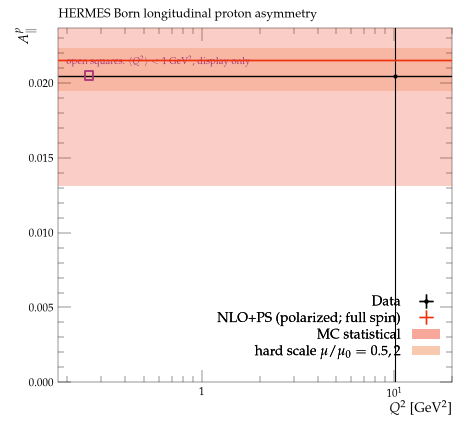
\includegraphics[width=0.48\textwidth]{figures/scan-20260722/hermes-legacy/d07-x01-y02.png}
  \hfill
  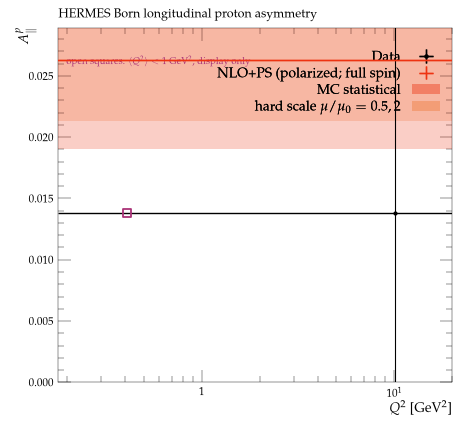
\includegraphics[width=0.48\textwidth]{figures/scan-20260722/hermes-legacy/d07-x02-y02.png}

  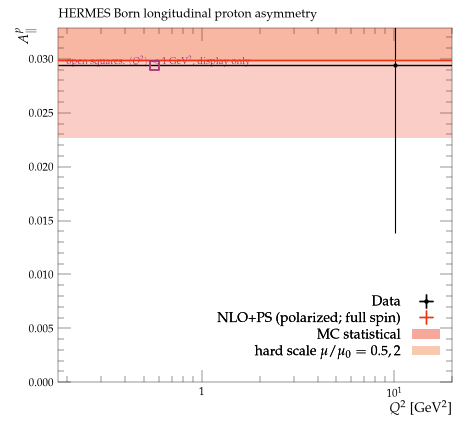
\includegraphics[width=0.48\textwidth]{figures/scan-20260722/hermes-legacy/d07-x03-y02.png}
  \hfill
  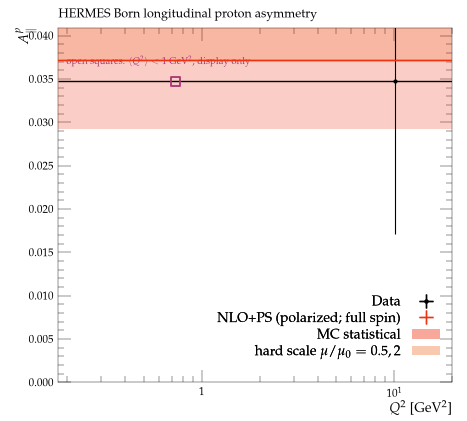
\includegraphics[width=0.48\textwidth]{figures/scan-20260722/hermes-legacy/d07-x04-y02.png}
  \caption{HERMES Born-level $A_\parallel^p(Q^2)$ for, from upper left to
  lower right, $0.0041<x<0.0073$, $0.0073<x<0.0118$,
  $0.0118<x<0.0168$, and $0.0168<x<0.0212$.  Open squares denote
  points with mean $Q^2<1\,\mathrm{GeV}^2$ and are display-only.  The red
  curve, Monte Carlo band and hard-scale envelope follow the conventions of
  fig.~\ref{fig:inclusive-dis-data}.}
  \label{fig:hermes-legacy-1}
\end{figure}

\begin{figure}[p]
  \centering
  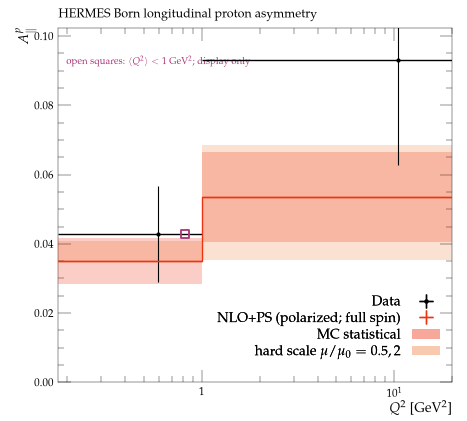
\includegraphics[width=0.48\textwidth]{figures/scan-20260722/hermes-legacy/d07-x05-y02.png}
  \hfill
  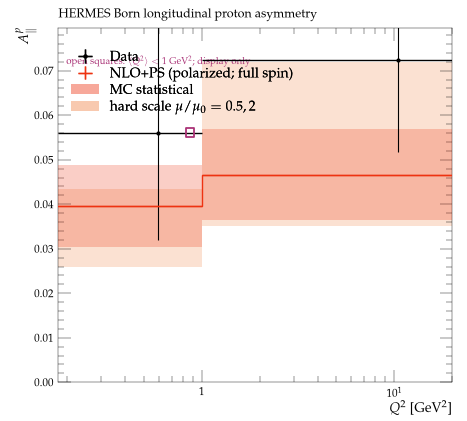
\includegraphics[width=0.48\textwidth]{figures/scan-20260722/hermes-legacy/d07-x06-y02.png}

  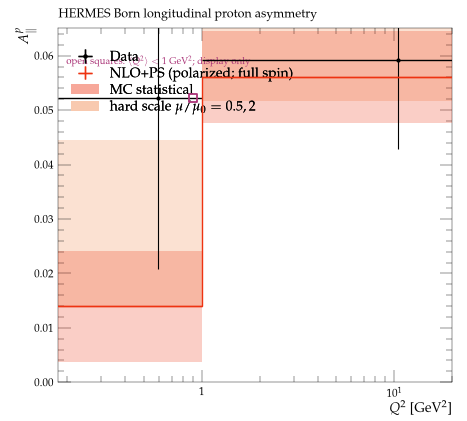
\includegraphics[width=0.48\textwidth]{figures/scan-20260722/hermes-legacy/d07-x07-y02.png}
  \hfill
  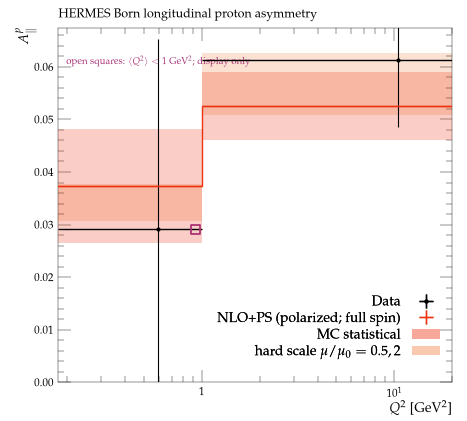
\includegraphics[width=0.48\textwidth]{figures/scan-20260722/hermes-legacy/d07-x08-y02.png}
  \caption{HERMES Born-level $A_\parallel^p(Q^2)$ for, from upper left to
  lower right, $0.0212<x<0.0295$, $0.0295<x<0.0362$,
  $0.0362<x<0.0444$, and $0.0444<x<0.0568$.  Marker and uncertainty
  conventions are those of fig.~\ref{fig:hermes-legacy-1}.}
  \label{fig:hermes-legacy-2}
\end{figure}

\begin{figure}[p]
  \centering
  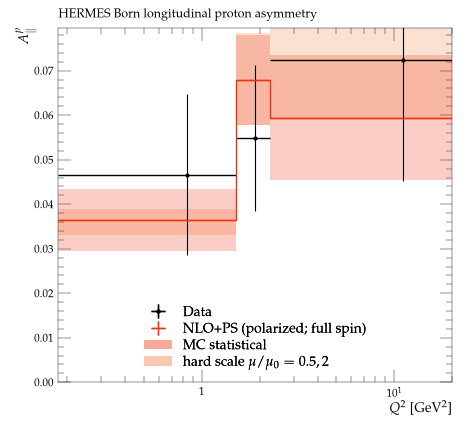
\includegraphics[width=0.48\textwidth]{figures/scan-20260722/hermes-legacy/d07-x09-y02.png}
  \hfill
  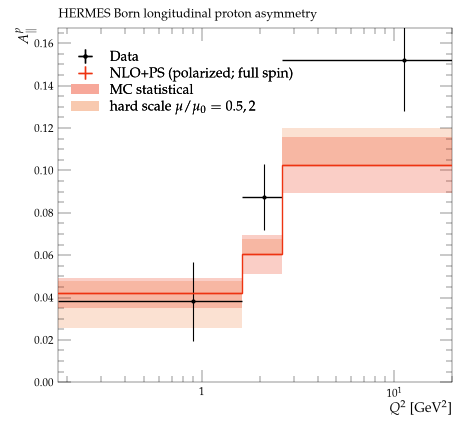
\includegraphics[width=0.48\textwidth]{figures/scan-20260722/hermes-legacy/d07-x10-y02.png}

  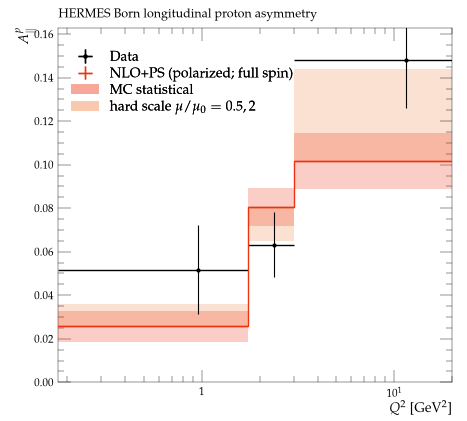
\includegraphics[width=0.48\textwidth]{figures/scan-20260722/hermes-legacy/d07-x11-y02.png}
  \hfill
  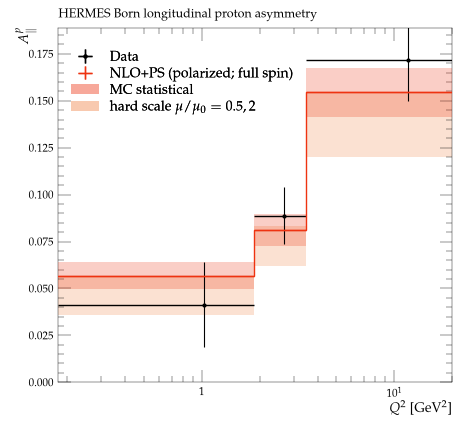
\includegraphics[width=0.48\textwidth]{figures/scan-20260722/hermes-legacy/d07-x12-y02.png}
  \caption{HERMES Born-level $A_\parallel^p(Q^2)$ for, from upper left to
  lower right, $0.0568<x<0.0727$, $0.0727<x<0.0929$,
  $0.0929<x<0.119$, and $0.119<x<0.152$.  Uncertainty conventions are
  those of fig.~\ref{fig:hermes-legacy-1}.}
  \label{fig:hermes-legacy-3}
\end{figure}

\begin{figure}[p]
  \centering
  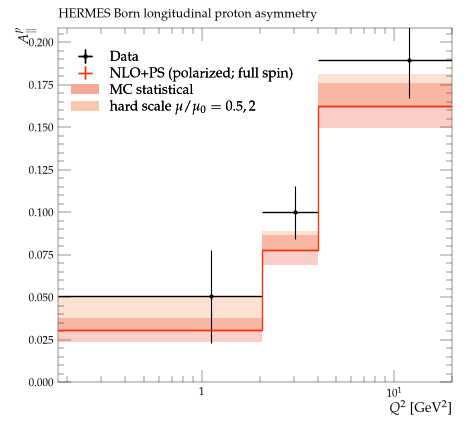
\includegraphics[width=0.48\textwidth]{figures/scan-20260722/hermes-legacy/d07-x13-y02.png}
  \hfill
  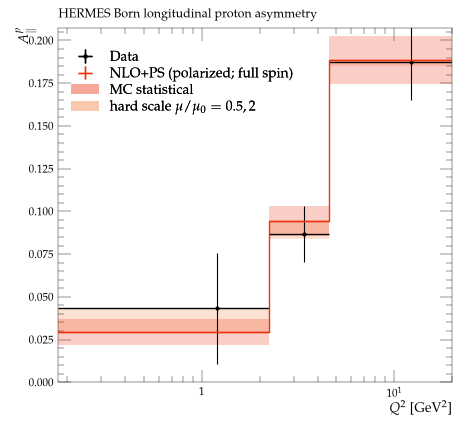
\includegraphics[width=0.48\textwidth]{figures/scan-20260722/hermes-legacy/d07-x14-y02.png}

  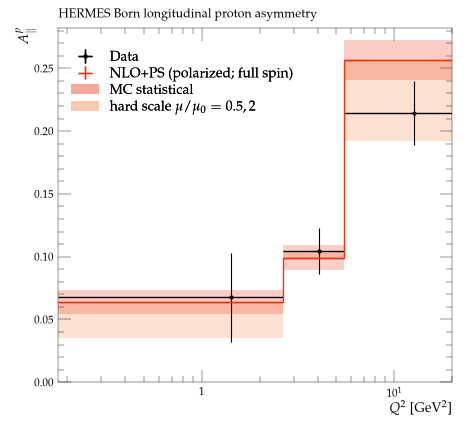
\includegraphics[width=0.48\textwidth]{figures/scan-20260722/hermes-legacy/d07-x15-y02.png}
  \hfill
  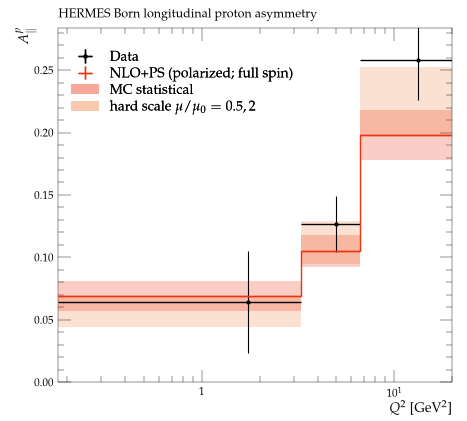
\includegraphics[width=0.48\textwidth]{figures/scan-20260722/hermes-legacy/d07-x16-y02.png}
  \caption{HERMES Born-level $A_\parallel^p(Q^2)$ for, from upper left to
  lower right, $0.152<x<0.194$, $0.194<x<0.249$,
  $0.249<x<0.318$, and $0.318<x<0.406$.  Uncertainty conventions are
  those of fig.~\ref{fig:hermes-legacy-1}.}
  \label{fig:hermes-legacy-4}
\end{figure}

\begin{figure}[p]
  \centering
  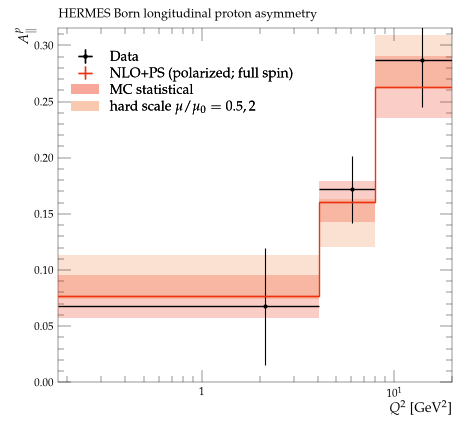
\includegraphics[width=0.48\textwidth]{figures/scan-20260722/hermes-legacy/d07-x17-y02.png}
  \hfill
  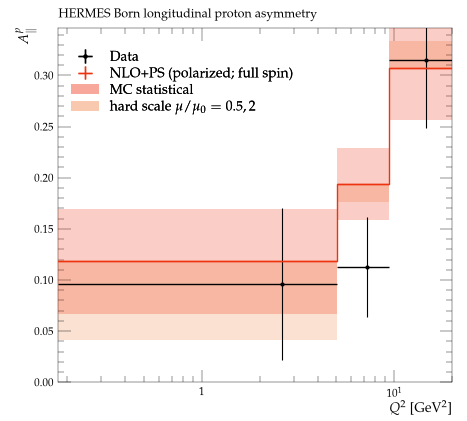
\includegraphics[width=0.48\textwidth]{figures/scan-20260722/hermes-legacy/d07-x18-y02.png}

  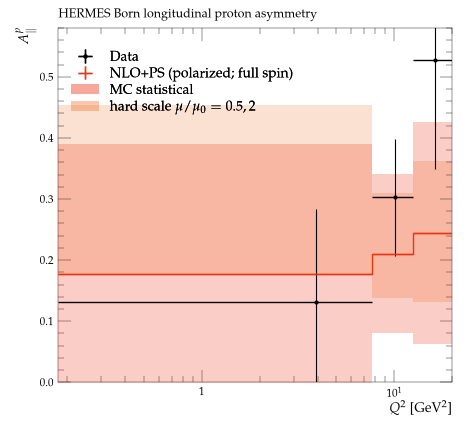
\includegraphics[width=0.48\textwidth]{figures/scan-20260722/hermes-legacy/d07-x19-y02.png}
  \caption{HERMES Born-level $A_\parallel^p(Q^2)$ for
  $0.406<x<0.520$ (upper left), $0.520<x<0.665$ (upper right), and
  $0.665<x<0.9$ (lower left).  Uncertainty conventions are those of
  fig.~\ref{fig:hermes-legacy-1}.}
  \label{fig:hermes-legacy-5}
\end{figure}

\clearpage
\section{Reproducibility summary}
\label{app:reproducibility}

\begin{table}[h]
  \centering
  \caption{Common simulation settings.  A check mark denotes inclusion in the
  nominal prediction.  The STAR jet observable is evaluated before
  hadronization even though the complete event is subsequently generated.}
  \footnotesize
  \setlength{\tabcolsep}{4pt}
  \begin{tabular}{@{}lccc@{}}
    \toprule
    Setting & DIS & STAR $W/Z$ & STAR jets \\
    \midrule
    hard accuracy & NLO POWHEG & LO & LO \\
    unpolarized PDF & NNPDF40 NLO & NNPDF40 NLO & NNPDF40 NLO \\
    polarized PDF & NNPDFpol2.0 NLO & NNPDFpol2.0 NLO & NNPDFpol2.0 NLO \\
    QCD shower & \checkmark & \checkmark & \checkmark \\
    QED shower & -- & \checkmark & -- \\
    spin-correlated evolution/decays & \checkmark & \checkmark & \checkmark \\
    hadronization and remnants & \checkmark & \checkmark & \checkmark \\
    multiple-parton interactions & -- & \checkmark & -- \\
    observable level & stable hadrons & stable leptons & hard shower partons \\
    hard-scale factors & $1/2,1,2$ & $1/2,1,2$ & $1/2,1,2$ \\
    \bottomrule
  \end{tabular}
\end{table}

\begin{table}[h]
  \centering
  \caption{Observable-specific assumptions and limitations.}
  \small
  \begin{tabular}{@{}p{0.23\textwidth}p{0.68\textwidth}@{}}
    \toprule
    Observable & Assumption or limitation \\
    \midrule
    HERMES and COMPASS $A_1$ & $A_2=g_2=0$; R1990 for HERMES and R1998 with finite-muon kinematics for COMPASS. \\
    HERMES SIDIS & Direct $A_\parallel$ comparison; deuteron impulse approximation with the 0.926 longitudinal factor; overlapping projections are assessed separately. \\
    HERMES low $Q^2$ & Scales are frozen at $1\GeV$; points with mean $Q^2<1\,\mathrm{GeV}^2$ are display-only. \\
    COMPASS 2010 & Fixed $160\GeV$ generation approximates the published 140--180 GeV beam selection; no unreported $W$ cut is imposed. \\
    COMPASS deuteron & Impulse approximation with effective nucleon polarization; no further nuclear correction. \\
    STAR weak bosons & LO hard matrix elements with NLO PDF inputs; the nominal full-event prediction includes MPI. \\
    STAR jets & LO hard matrix elements with NLO PDF inputs; hard shower-parton jets and MPI off define the publication-level comparison. \\
    Displayed scan & Central PDF members and hard-scale variations only; the PDF-replica bands remain to be generated. \\
    PDF comparison & NNPDFpol2.0 contains much of the compared information, so agreement is not an independent PDF validation. \\
    \bottomrule
  \end{tabular}
\end{table}

\bibliographystyle{JHEP}
\bibliography{references}

\end{document}
